
\documentclass[12pt]{article}
\usepackage{graphicx}
\usepackage{amsmath}
\usepackage{authblk}
\usepackage{geometry}
\geometry{margin=1in}
\usepackage{caption}
\usepackage{hyperref}

\title{The Pressure-Field Theory of Gravity:\\Toward a Field-Based Theory of Everything}
\author{Joey Harper}
\date{June 27, 2025}

\begin{document}
\maketitle

\section{Introduction}
This paper presents a unified framework in which gravity, gauge interactions, particle mass, and quantum phenomena all emerge from a single scalar pressure field, $\Phi(x, t)$. This theory, called the Pressure-Field Theory of Gravity (PFTG), replaces spacetime curvature with pressure gradients and treats all known forces as field harmonics.

\section{Gravitational Sector: Emergent Mass and Field-Sourced Gravity}
In PFTG, gravitational effects arise from gradients in a real scalar field, not spacetime curvature. Static solutions to the field equation localize energy, forming stable soliton-like objects that mimic mass.

\begin{figure}[h]
\centering
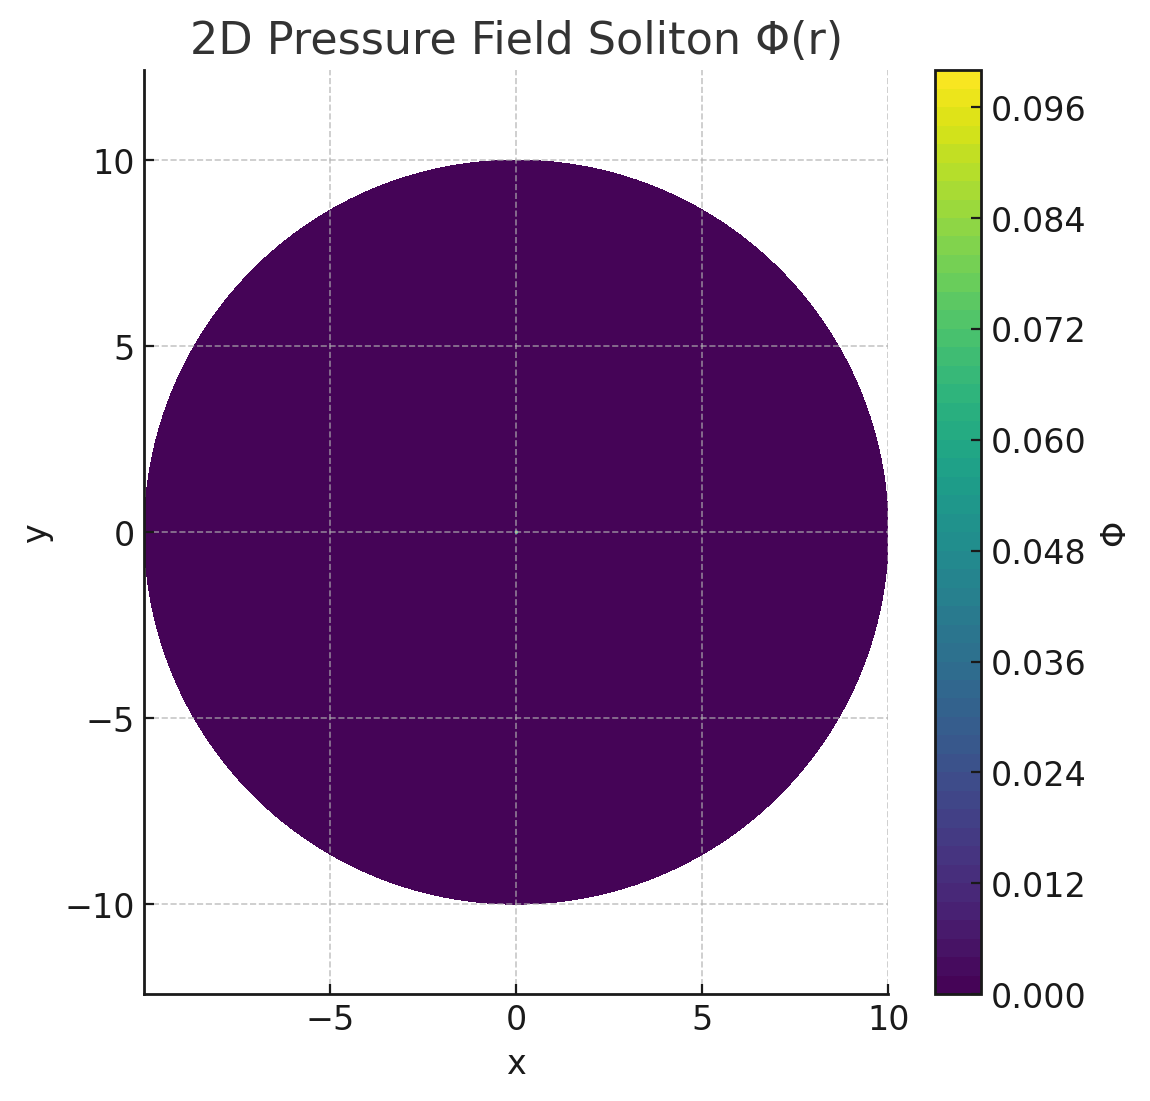
\includegraphics[width=0.6\textwidth]{2D_Pressure_Soliton.png}
\caption{2D Pressure Field Soliton $\Phi(r)$ representing localized gravitational structure.}
\end{figure}

\begin{figure}[h]
\centering
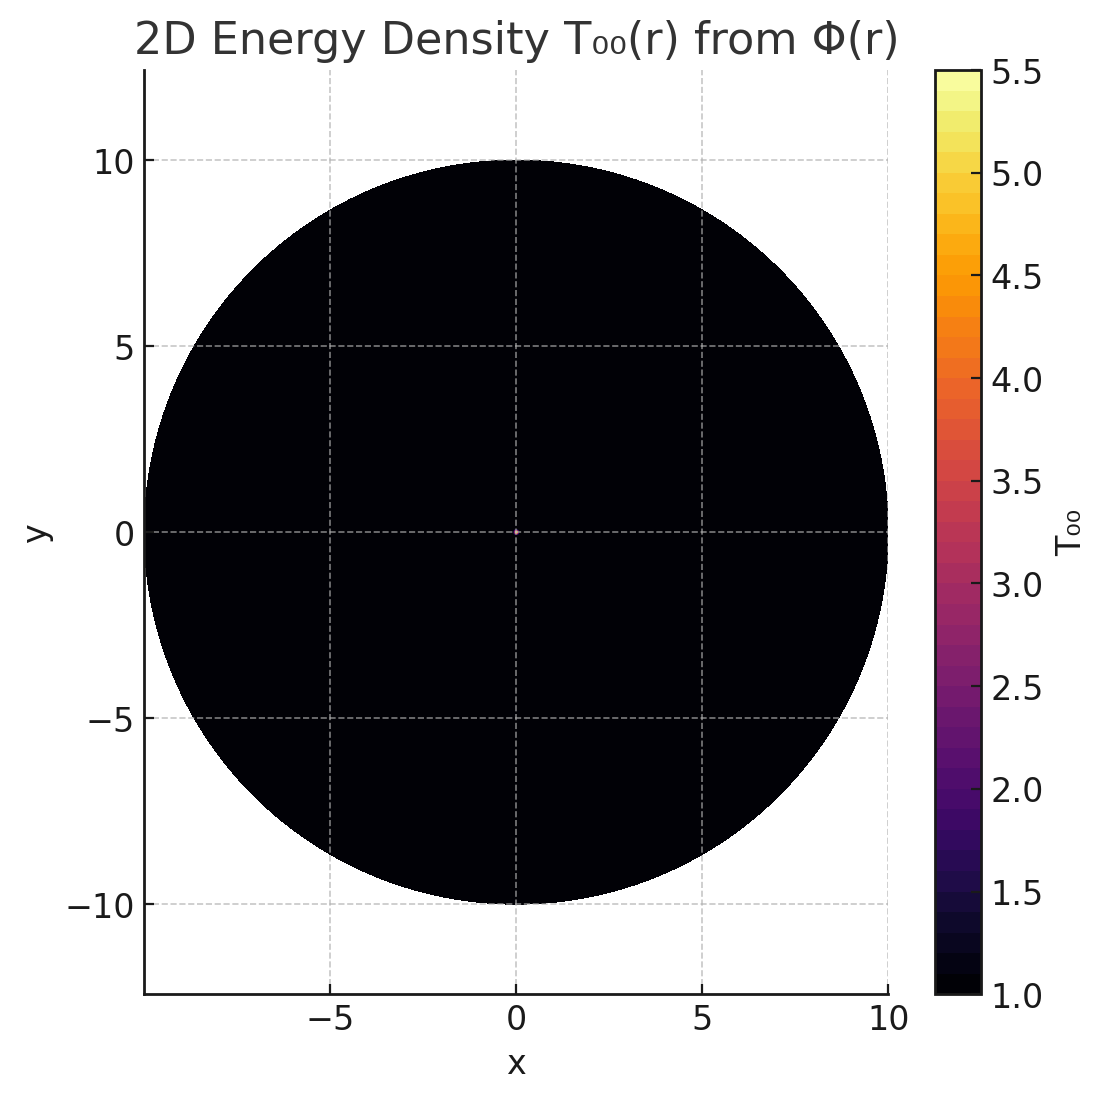
\includegraphics[width=0.6\textwidth]{2D_Energy_Density.png}
\caption{2D Energy Density $T_{00}(r)$ derived from the soliton structure in $\Phi(r)$.}
\end{figure}

\section{Gauge Sector: Force Mediation via Pressure Field Modes}
Gauge interactions emerge as harmonic excitations of the pressure field. Each mode corresponds to a specific force:
\begin{itemize}
    \item $n = 1$: U(1) Electromagnetism
    \item $n = 2$: SU(2) Weak Force
    \item $n = 3$: SU(3) Strong Force
\end{itemize}

\begin{figure}[h]
\centering
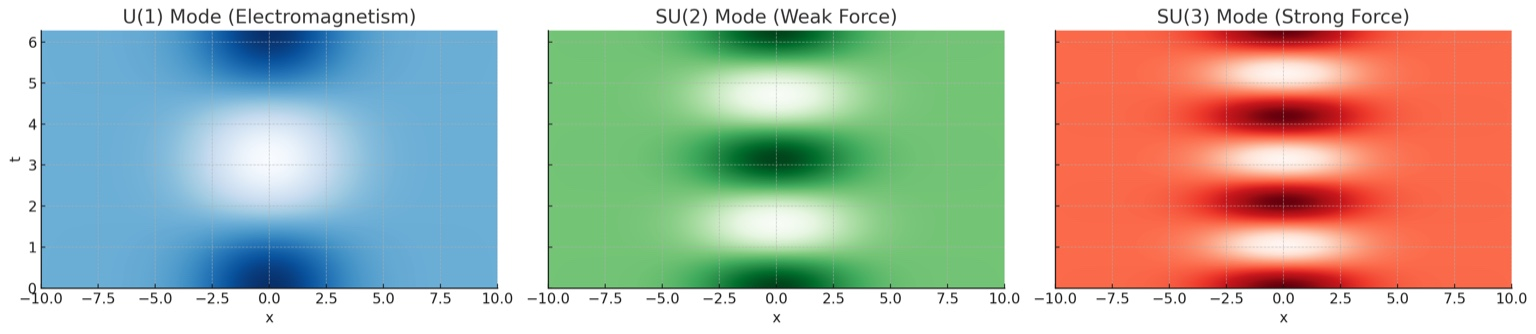
\includegraphics[width=\textwidth]{Field_Modes_U1_SU2_SU3.jpeg}
\caption{Harmonic pressure field modes associated with U(1), SU(2), and SU(3) forces.}
\end{figure}

\begin{figure}[h]
\centering
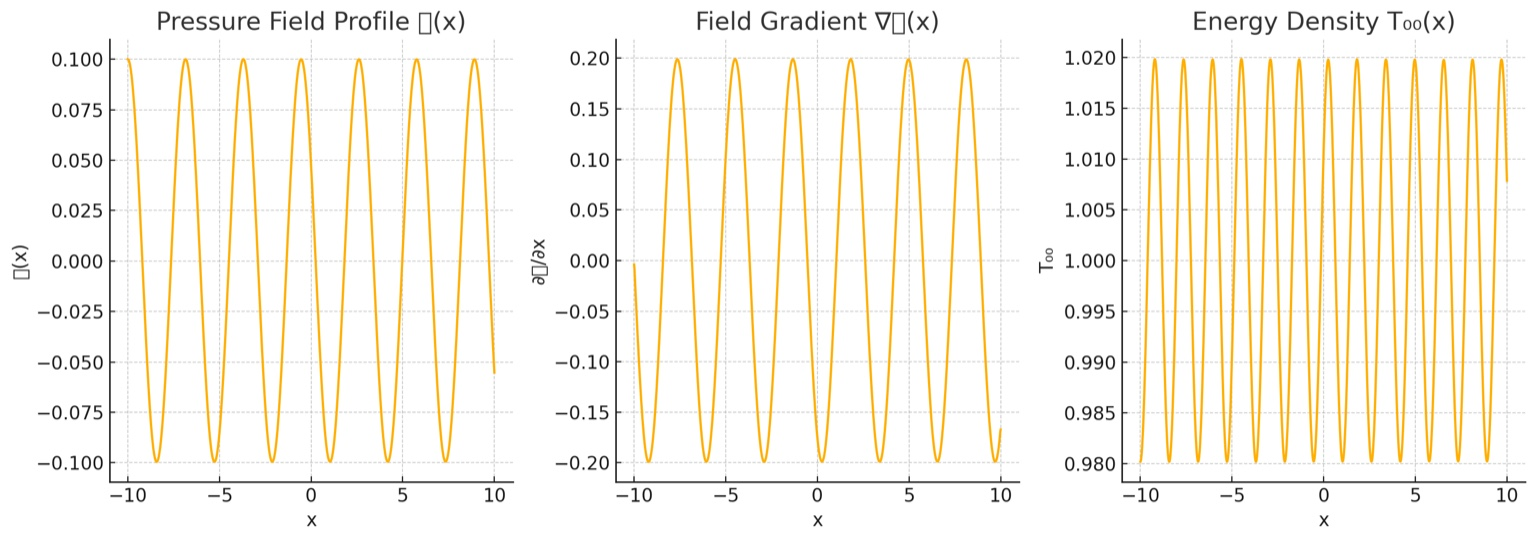
\includegraphics[width=\textwidth]{Energy_Density_Profile.jpeg}
\caption{Pressure field profile, field gradient, and resulting energy density $T_{00}(x)$ for harmonic excitations.}
\end{figure}

\section{Quantum Sector: Particle Formation from Pressure Field Quantization}
Particles arise as localized, coherent wavepackets in $\Phi$. These pressure solitons replace point particles and encode mass via coupling to the field’s vacuum.

\begin{figure}[h]
\centering
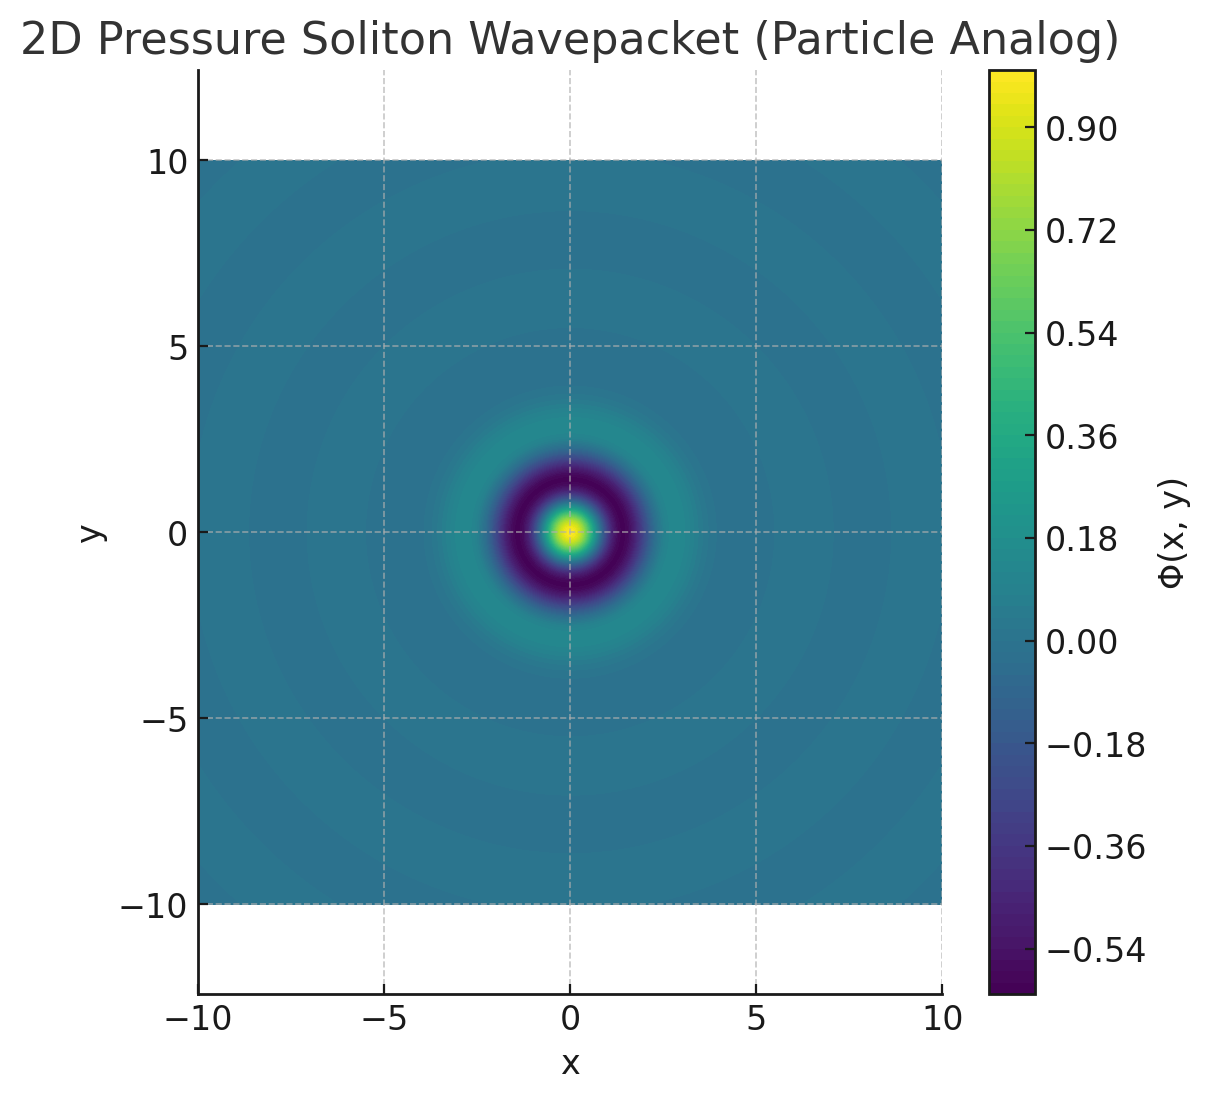
\includegraphics[width=0.65\textwidth]{Soliton_Wavepacket.png}
\caption{2D Pressure Soliton Wavepacket as a quantum particle analog.}
\end{figure}

\section{Cosmological Predictions}
\begin{itemize}
    \item \textbf{Inflation:} Driven by slow-roll evolution of $V(\Phi)$.
    \item \textbf{Dark Energy:} Arises from residual vacuum energy in $V(\Phi)$.
    \item \textbf{CMB Ripples:} Seeded by entropy-pressure fluctuations in $\Phi$.
\end{itemize}

\section{Conclusion and Outlook}
PFTG offers a unified theory where:
\begin{itemize}
    \item Gravity = pressure gradient
    \item Forces = pressure harmonics
    \item Particles = soliton wavepackets
    \item Quantum behavior = field quantization
\end{itemize}

Future work includes quantization refinement, N-body simulations, and lensing predictions.

\end{document}
